\documentclass[12pt,a4paper]{book}
\usepackage[utf8]{inputenc}
\usepackage{amsmath}
\usepackage{amsfonts}
\usepackage{amssymb}
\usepackage{graphicx}
\usepackage{tikz}
\begin{document}
	
	%%%%=============================Ống nghiệm cơ bản
	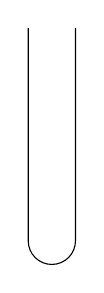
\begin{tikzpicture}
		%\draw[step=1,gray,very thin](-2,-1) grid (12,10);
		%\draw[->](-2,0)--(13,0) node [below] {$x$};
		%\draw[->](0,-1)--(0,1) node [left] {$y$};
		%\foreach \x in {-2,...,12}
		%\draw (\x,0.1)--(\x,-0.1) node [below] {\x};
		%\foreach \y in {-1,...,10} % Hai số -2, -1 này cần chia vạch và ghi số
		%\draw[shift={(0,\y)},color=black] (2pt,0pt) -- (-2pt,0pt) node[left] {\normalsize $\y$}; %Chia vạch và ghi số bên trái
		\begin{scope}[xshift=0,yshift=0]
			\draw (0,3)--(0,0.3) arc (-180:0:0.3)--(0.6,3); %ống nghiệm 2
		\end{scope}
	\end{tikzpicture}
	
	%%%%=========================Ống nghiệm có nút cao su
	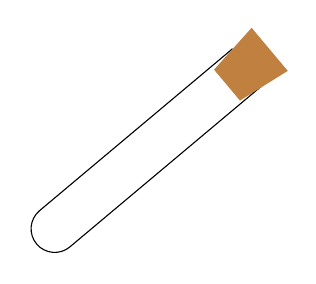
\begin{tikzpicture}
		\begin{scope}[xshift=-2cm,yshift=2cm,rotate=-50]%ống nghiệm 
			\draw (0,3.5)--(0,0.3) arc (-180:0:0.3)--(0.6,3.5); 
		\end{scope}
		\begin{scope}[xshift=0.75cm,yshift=4.1cm,rotate=-50]%%nút cao su
			\filldraw[brown] (-0.2,0.4)--++(0.1,-0.7)--++(0.5,0)--++(0.1,0.7);
		\end{scope}
	\end{tikzpicture}
	
	
	%%%%================%%ỐNG NGHIỆM CÓ DUNG DỊCH
	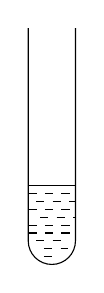
\begin{tikzpicture}%%ỐNG NGHIỆM CÓ DUNG DỊCH
		%\draw[step=1,gray,very thin](-2,-1) grid (12,10);
		%\draw[->](-2,0)--(13,0) node [below] {$x$};
		%\draw[->](0,-1)--(0,1) node [left] {$y$};
		%\foreach \x in {-2,...,12}
		%\draw (\x,0.1)--(\x,-0.1) node [below] {\x};
		%\foreach \y in {-1,...,10} % Hai số -2, -1 này cần chia vạch và ghi số
		%draw[shift={(0,\y)},color=black] (2pt,0pt) -- (-2pt,0pt) node[left] {\normalsize $\y$}; %Chia vạch và ghi số bên trái
		%%%%==========Vẽ ống nghiệm
		\begin{scope}[xshift=0,yshift=0cm]%ống nghiệm 
			\draw (0,3)--(0,0.3) arc (-180:0:0.3)--(0.6,3);
			\draw (0,1)--(0.6,1);
			\draw [dashed] (0,0.9)--(0.6,0.9) (0.1,0.8)--(0.6,0.8) (0,0.7)--(0.6,0.7) (0.15,0.6)--(0.6,0.6) (0,0.5)--(0.6,0.5) (0,0.4)--(0.6,0.4) (0.1,0.3)--(0.5,0.3) (0.2,0.2)--(0.5,0.2) (0.2,0.1)--(0.4,0.1);
		\end{scope}
		%
	\end{tikzpicture}
	
	%%%%%%%%%%%%%%%%%%%ỐNG NGHIỆM CÓ DUNG DỊCH và chất rắn
	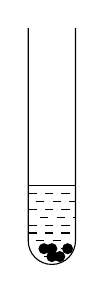
\begin{tikzpicture}%%ỐNG NGHIỆM CÓ DUNG DỊCH và chất rắn
		%\draw[step=1,gray,very thin](-2,-1) grid (12,10);
		%\draw[->](-2,0)--(13,0) node [below] {$x$};
		%\draw[->](0,-1)--(0,1) node [left] {$y$};
		%\foreach \x in {-2,...,12}
		%\draw (\x,0.1)--(\x,-0.1) node [below] {\x};
		%\foreach \y in {-1,...,10} % Hai số -2, -1 này cần chia vạch và ghi số
		%\draw[shift={(0,\y)},color=black] (2pt,0pt) -- (-2pt,0pt) node[left] {\normalsize $\y$}; %Chia vạch và ghi số bên trái
		%%%==========Vẽ ống nghiệm
		\begin{scope}[xshift=0,yshift=0cm]%ống nghiệm 
			\draw (0,3)--(0,0.3) arc (-180:0:0.3)--(0.6,3);
			\draw (0,1)--(0.6,1);
			\draw [dashed] (0,0.9)--(0.6,0.9) (0.1,0.8)--(0.6,0.8) (0,0.7)--(0.6,0.7) (0.15,0.6)--(0.6,0.6) (0,0.5)--(0.6,0.5) (0,0.4)--(0.6,0.4) (0.1,0.3)--(0.5,0.3) (0.2,0.2)--(0.5,0.2) (0.2,0.1)--(0.4,0.1);
			\foreach \x/\y in {0.3/0.1,0.4/0.1,0.5/0.2,0.3/0.2,0.2/0.2}\fill (\x,\y) circle (2pt) ;
		\end{scope}
		
	\end{tikzpicture}
	
\end{document}